\documentclass[aspectratio=169]{beamer}
\usetheme{Madrid}
 
\usepackage{graphicx}
\usepackage[spanish]{babel}
\usepackage[utf8]{inputenc}

%\setbeamertemplate{footline}[frame number]

\begin{document}

\title{
	\textbf{Introduction to neural networks}} 
\subtitle{Parametric models} 
\author[J.I. Vasquez]{\textbf{Juan Irving Vásquez}}
%\date{December 2020 \copyright} 
\date{\today}
\institute[jivg.org]{ Instituto Politécnico Nacional \\Centro de Innovación y Desarrollo Tecnológico en Cómputo\\ jivg.org}
% logo of my university
\titlegraphic{
\includegraphics[height=1.2cm]{ipn-cidetec.png}\hspace{0.1cm}
\includegraphics[height=1.2cm]{escudoESCOM}}

%{ 	\usebackgroundtemplate{
\includegraphics[width=1.0\paperwidth]{fondo}}%
\frame{\titlepage} 
%}

\begin{frame}
\frametitle{Overview} 
\tableofcontents
\end{frame}

\section{Parametric models}

\begin{frame}{Parametric models}
\begin{figure}
    \centering
    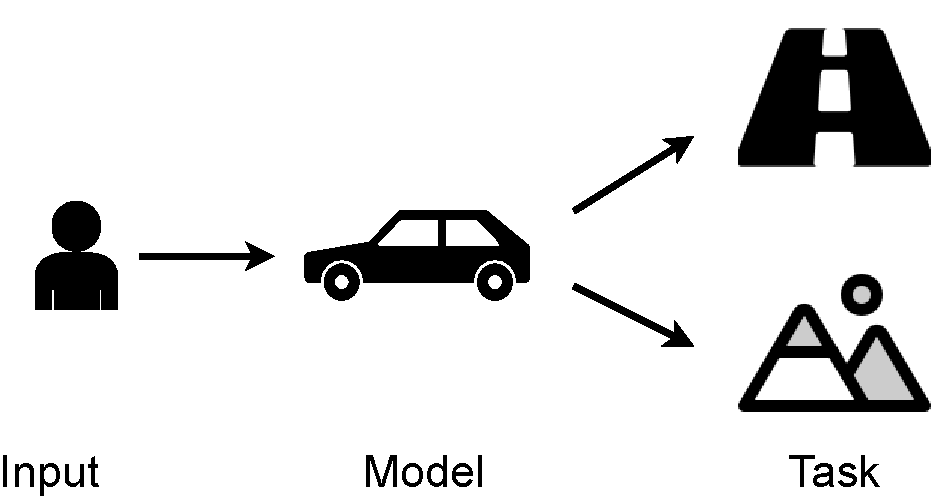
\includegraphics[width=0.6\textwidth]{parametric model.drawio.pdf}
    %\caption{Caption}
    %\label{fig:my_label}
\end{figure}
\end{frame}

\begin{frame}{Parametric models}
	\framesubtitle{Features}
	\begin{block}{Parametric model}
		A learning model that summarizes data with a set of parameters of fixed size is called a parametric model [Russell and Norvig].
	\end{block}
	\begin{itemize}
		\item Reduces the data spatial complexity
		\item Standardizes the training algorithms
		\item To define the model size is a new problem
	\end{itemize}
\end{frame}


\begin{frame}{Parametric models}
%\framesubtitle{Line equation}
General model:
    \begin{equation}
    	\hat{Y} = \Phi_{\theta}(X)
    \end{equation}
Example
	\begin{equation}
		y = mx + b
	\end{equation}
	\begin{equation}
		\theta = ?
	\end{equation}
\end{frame}


\begin{frame}{Nonparametric models}
\begin{columns}
	\begin{column}{0.5\textwidth}
    \begin{itemize}
	\item A nonparametric model is one that can not be characterized by a bounded set of parameters. 
	\begin{itemize}
		\item E.g. instance based learning
		\item Nearest neighbors
		\item Nonparametric regression
	\end{itemize}
\end{itemize}
	\end{column}
\pause
	\begin{column}{0.5\textwidth}  %%<--- here
%\begin{figure}
%	\centering
	
\includegraphics[height=0.8\textheight]{iaif}
%	\caption{}
%	\label{fig:iaif}
%\end{figure}
	\end{column}
\end{columns}	
\end{frame}


\section{Nonparametric models}

\begin{frame}
\frametitle{References}
{\footnotesize
\begin{itemize}
    \item RUSSELL, Stuart J.; NORVIG, Peter. Inteligencia Artificial: un enfoque moderno. Capítulo 18 Learning from examples. 2004.
	\item Photo by Tommy Lisbin on Unsplash
	\item Photo by Hanson Lu on Unsplash
\end{itemize}
}
\end{frame}
%
%


\end{document}